\renewcommand{\thesection}{\Alph{section}}
\setcounter{figure}{0}
\renewcommand{\thefigure}{\Alph{section}.\arabic{figure}}
\appendix
\addchap{Anhang}

\captionsetup{list=false}

\section{Bilder}
\begin{figure}[H]
\centering
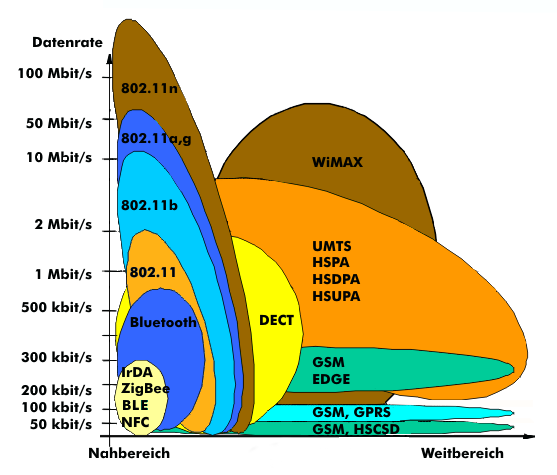
\includegraphics[scale=1]{Bilder/Funktechnologien.png} 
\caption{Überblick zu heutigen Funktechnologien \cite{FUE}}
\label{fig:FUE}
\end{figure}
\begin{figure}[H] 
\centering
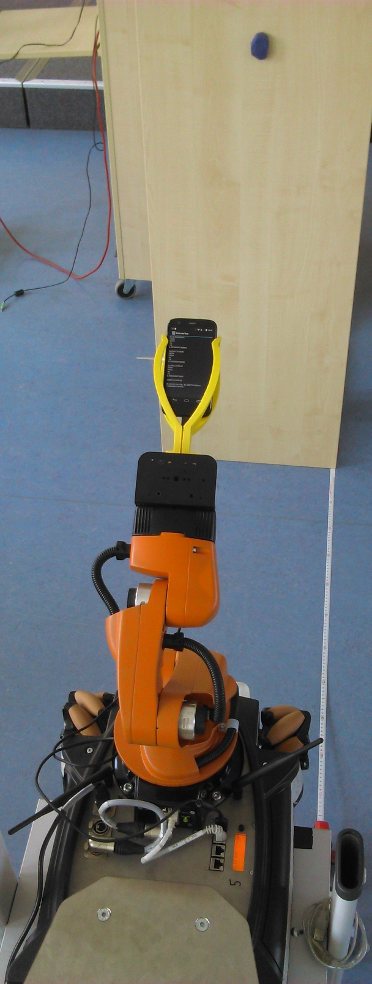
\includegraphics[scale=0.3]{Bilder/MessungDistanz1}
\caption{Distanz-Signalstärke-Messung Bild 1}
\label{fig:MessungDistanz1}
\end{figure}
\begin{figure}[H] 
\centering
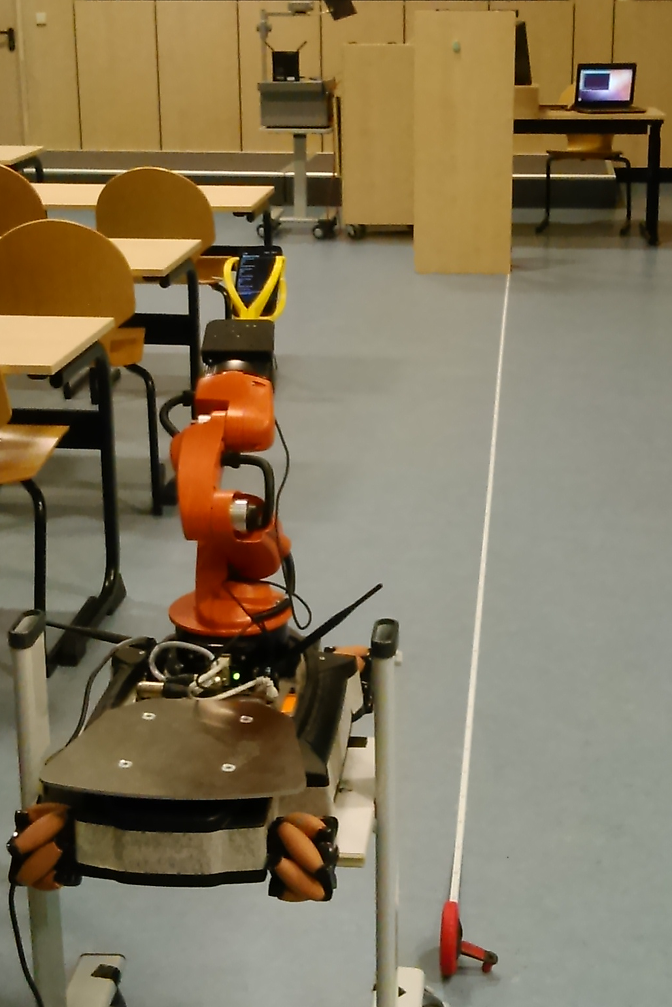
\includegraphics[scale=0.3]{Bilder/MessungDistanz2}
\caption{Distanz-Signalstärke-Messung Bild 2}
\label{fig:MessungDistanz2}
\end{figure}
\begin{figure}[H] 
\centering
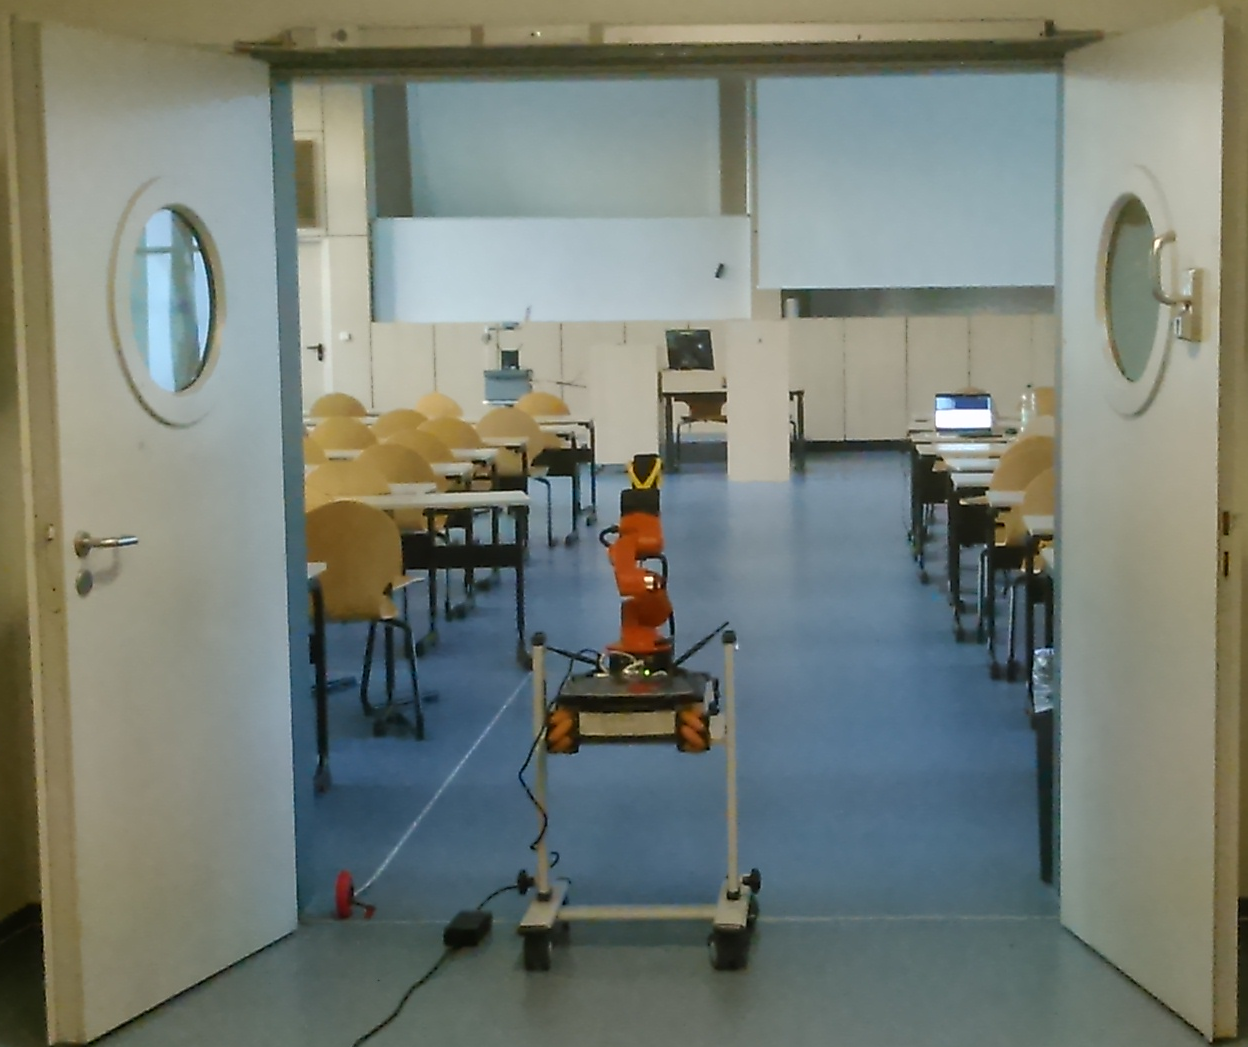
\includegraphics[scale=0.3]{Bilder/MessungDistanz3}
\caption{Distanz-Signalstärke-Messung Bild 3}
\label{fig:MessungDistanz3}
\end{figure}